\chapter{Estimação de Densidade por Núcleo}\label{cap:kde}

O \ac{KDE} é uma técnica não-paramétrica para estimação de densidades, onde cada observação é ponderada pela distância em relação a um valor central, o núcleo. Após a estimação da densidade de um conjunto de dados, tem-se conhecimento sobre a probabilidade de ocorrência de cada evento, o que possibilita análises sobre essas observações e, por exemplo, a aplicação deste método em problemas de classificação \cite{kernelthesis}.

Nas próximas seções, os métodos univariado e multivariado serão descritos, bem como os critérios de otimização dos mesmos.

\section{Estimação de densidade univariada}\label{sec:kdeuni}

\subsection{Histograma para KDE}

Uma das maneiras mais simples de abordar esse problema, muito utilizada na literatura, é a estimação por histograma, mostrada na equação~\ref{eq:4T01}:

\begin{equation}\label{eq:4T01}
{\hat f_h}\left( x \right) = \frac{1}{{nh}}\sum\limits_{i = 1}^n {\sum\limits_j {I\left( {{x_i} \in {B_j}} \right)I\left( {x \in {B_j}} \right)} }
\end{equation}

Onde, $n$ é o número de eventos, $i$ e $j$ são os subíndices de eventos, $I$ é a função indicadora e,

\begin{equation}\label{eq:4T02}
\begin{array}{l}
 {B_j} = \left[ {{x_o} + \left( {j - 1} \right)h,{x_o} + jh} \right) \\
 j \in {\rm{Z}} \\
 \end{array}
\end{equation}

Esse método lida com os parâmetros de origem (${x_o}$) e tamanho do \emph{bin} (\emph{h}), sendo que ambos, se escolhidos de maneira errada, podem resultar em uma má estimação. No intuito de diminuir esse problema, é possível efetuar a estimação pela média de sub-histogramas, tornando o método independente da origem ${x_o}$ \cite{seather1992performance}, como mostra a equação~\ref{eq:4T03}.

\begin{equation}\label{eq:4T03}
{\hat f_h}\left( x \right) = \frac{1}{M}\sum\limits_{l = 0}^{M - 1} {\frac{1}{{nh}}\sum\limits_{i = 1}^n {\sum\limits_j {I\left( {{x_i} \in {B_j}} \right)I\left( {x \in {B_j}} \right)} } }
\end{equation}

Onde,

\begin{equation}\label{eq:4T04}
\begin{array}{l}
 {B_{j,l}} = \left[ {\left( {j - 1 + \frac{1}{M}} \right)h,\left( {j + \frac{1}{M}} \right)h} \right) \\
 l \in \left\{ {0,1,...,M - 1} \right\} \\
 \end{array}
\end{equation}

Essa configuração produz uma estimação mais suave que o histograma, mas é somente uma maneira melhor de utilizar esse conceito básico, podendo não resultar em uma boa representação da densidade. Entretanto, o problema de otimização do parâmetro $h$ continua e sua otimização foi considerada em vários trabalhos, como por exemplo: \cite{chen2002robust}, \cite{abramson1982bandwidth}, \cite{comaniciu2001variable}, \cite{silverman1986density} e \cite{jones1991roles}.

\subsection{Modelo do Estimador de Densidade por Núcleo}

O KDE, de forma direta, aplica uma função de \emph{Kernel} em cada evento, levando em conta a contagem de eventos em sua vizinhança. O estimador é dado pela equação~\ref{eq:4T05} e foi Rosenblatt em 1956 o primeiro autor que considerou esse modelo.

\begin{equation}\label{eq:4T05}
    \hat f\left( {{x_i}} \right) = \frac{1}{{nh}}\mathop \sum \limits_{k = 1}^{N} K\left( {\frac{{({x_i} - {X_k})}}{h}} \right)
\end{equation}
onde \emph{K(u)} é a função \emph{Kernel} e o parâmetro \emph{h} é conhecido como largura de banda.

Para garantir que esse modelo retorne uma função de densidade, o \emph{Kernel} deve satisfazer $\mathop \smallint \limits_{ - \infty }^{ + \infty } K\left( u \right)du = 1$ e $\begin{array}{*{20}{c}}
   {K\left( u \right) \ge 0} & \forall  & {u \in \Re }  \\
\end{array}$ (Funções Kernels de ordem maiores que 2 não satisfazem a última propriedade).

Algumas outras propriedades da função Kernel são:

\begin{itemize}
  \item $K\left( u \right) = K\left( { - u} \right)$ ;
  \item $K\left( u \right)$ tem seu máximo quando $u=0$;
  \item Os momentos do \emph{kernel} são: ${k_j}(k) = \mathop \smallint \limits_{ - \infty }^{ + \infty } {u^j}K\left( u \right)du$;
  \item A ordem do \emph{kernel} \emph{v} é definida como a ordem do primeiro momento não nulo.
\end{itemize}

Alguns exemplos de funções \emph{kernel} de segunda ordem são mostradas abaixo, sendo que a função Gaussiana foi a escolhida para esse trabalho:

\begin{itemize}
  \item Triangular:  $K\left( u \right) = (1 - |u|)I(|u| \le 1)$
  \item Epanechnikov: $K\left( u \right) = \frac{3}{4}(1 - u)I(|u| \le 1)$
  \item Quartic (Biweight): $K\left( u \right) = \frac{{15}}{{16}}(1 - u)I(|u| \le 1)$
  \item Triweight: $K\left( u \right) = \frac{{35}}{{32}}(1 - u)I(|u| \le 1)$
  \item Gaussiana: $K\left( u \right) = \frac{1}{{\sqrt {2\pi } }}{e^{\left( { - \frac{1}{2}u} \right)}}$
\end{itemize}

%A relação entre estimação de densidade via histograma e \emph{kernel} surge do fato do uso da função \emph{kernel} triangular ser comparável a utilizar o método por histogramação no seu limite, quando $M \to \infty $.

Em ambas as abordagens, histogramação e KDE, fica clara a dependência da estimação em relação ao parâmetro $h$ de largura de banda. Nas próximas seções, serão discutidos os critérios para otimização da estimação de densidade e, consequentemente, da escolha ótima do parâmetro $h$.

\subsection{Critério de Otimização}

No que tange a otimização de estimadores de densidade, não existe uma maneira geral de otimização; toda otimização é feita olhando de maneira particular para um certo critério \cite{kernelthesis}. Essa seção tem o intuito de mostrar alguns métodos de otimização de estimadores e suas propriedades.

\subsubsection{Critério Baseado na Distância ${L_1}$}

Um ideia bastante comum para medir a diferença entre duas funções quaisquer $f$ e $g$ é utilizando o método ${L_p}$ \cite{kernelthesis}, definido como:

\begin{equation}\label{eq:4T06}
   {L_p} = {\left( {\int {{{\left| {f - g} \right|}^p}} } \right)^{{\raise0.7ex\hbox{$1$} \!\mathord{\left/
 {\vphantom {1 p}}\right.\kern-\nulldelimiterspace}
\!\lower0.7ex\hbox{$p$}}}}
\end{equation}

Onde $p$ é o parâmetro a ser escolhido. No caso mais simples, $p=1$, a equação~\ref{eq:4T06} se torna a equação~\ref{eq:4T15}.

\begin{equation}\label{eq:4T15}
{L_1} = {\int {\left| {f - g} \right|} }
\end{equation}

A equação~\ref{eq:4T15} é chamado de \ac{IAE} e deve ser minimizada, no intuito de garantir uma boa estimação da densidade.

\subsubsection{Critério Baseado na Distância ${L_2}$}\label{sec:mise}

Quando $p=2$ é escolhido na equação~\ref{eq:4T06}, temos:

\begin{equation}\label{eq:4T07}
ISE\left( {{{\hat f}_h}} \right) = \int {{{\left[ {{{\hat f}_h}\left( x \right) - f\left( x \right)} \right]}^2}dx}
\end{equation}

A equação~\ref{eq:4T07} é então chamada de \ac{ISE}, sendo assim, para o cálculo do \ac{MISE}, utiliza-se o valor esperado de $f\left( x \right)$, equação~\ref{eq:4T08}. Em \cite{jones1991roles}, o autor faz uma comparação do uso desses dois métodos e conclui que encontrar o valor otimizado da largura de banda utilizando o MISE apresenta melhores resultados que por ISE.

\begin{equation}\label{eq:4T08}
MISE\left( {{{\hat f}_h}} \right) = \int {E{{\left\{ {{{\hat f}_h}\left( x \right) - f\left( x \right)} \right\}}^2}dx}
\end{equation}

Do mesmo modo que o \ac{MSE}, que é a medida do erro médio de um certo ponto $x$, a expressão do MISE pode ser decomposta em termos de \emph{bias} e variância. A partir dessa decomposição, existem na literatura muitos estudos sobre a minimização dos critério MISE, alguns deles serão abordados na Seção~\ref{sec:amise}.

\subsubsection{Critério Baseado na Distância ${L_\infty }$}

De acordo com a equação~\ref{eq:4T06}, qualquer valor de $p$ pode ser escolhido. Entretanto, para escolhas de $p$ maiores que dois, não existem propriedades muito úteis, no sentido de otimização de estimadores. Sendo assim, para $p > 2$, o único caso que pode ser interessante é quando $p \to \infty $, que é igual a minimizar o erro máximo absoluto entre duas funções, $f$ e $g$ por exemplo \cite{kernelthesis}.

Todas as medidas descritas são estritamente critérios matemáticos, que fazem medidas, de modos diferentes, de similaridade entre duas funções. Entretanto, essas medidas podem não levar ao tipo de otimização desejada para estimadores de densidade. Como exemplo, o critério ${L_\infty }$, que ignora as caudas da distribuição, sendo que essas tornam-se mais importantes à medida em que se aumenta o número de dimensões.

\subsection{Cálculo dos critérios de erro}\label{sec:amise}


\subsubsection{MISE e AMISE}\label{sec:fixed}

%Um problema do MISE é o fato de depender da largura de banda ($h$), entretanto, existe uma maneira de superar esse problema com o uso de aproximações do bias e da variância \cite{wandkernel}, efetuando algumas suposições:
%
%\begin{equation}\label{eq:4T09}
%\begin{array}{l}
% \mathop {\lim }\limits_{n \to \infty } h = 0 \\
% \mathop {\lim }\limits_{n \to \infty } nh = \infty  \\
% \end{array}
%\end{equation}
%
%O que significa que o parâmetro $h$ aproxima de zero a taxas mais lentas que ${n^{ - 1}}$.

Como introduzido na Seção~\ref{sec:mise}, o MSE pode ser dividido em dois termos, como mostrado na equação~\ref{eq:4T16}:

\begin{equation}\label{eq:4T16}
\begin{array}{ccl}
 MSE\left( {{{\hat f}_h}} \right) &=& E{\left\{ {{{\hat f}_h}\left( x \right) - f\left( x \right)} \right\}^2} \\
  &=& Bias{\left( {{{\hat f}_h}\left( x \right)} \right)^2} + {\mathop{\rm var}} \left( {f\left( x \right)} \right) \\
 \end{array}
\end{equation}

\paragraph{Estimação do \emph{Bias}}

Sabendo que o valor esperado da transformação por \emph{kernel} pode ser escrita como:

\begin{equation}\label{eq:4T17}
E\left\{ {\hat f\left( x \right)} \right\} = \int {\frac{1}{h}K\left( {\frac{{(z - x)}}{h}} \right)} f\left( z \right)dz
\end{equation}
usando uma mudança de variáveis, $u = {{\left( {z - x} \right)} \mathord{\left/
 {\vphantom {{\left( {z - x} \right)} h}} \right.
 \kern-\nulldelimiterspace} h}$ , temos:

\begin{equation}\label{eq:4T18}
E\left\{ {\hat f\left( x \right)} \right\} = \int {K\left( u \right)} f(x + hu)du
\end{equation}

A equação~\ref{eq:4T18} mostra que o valor esperado é a média de $f(z)$ localmente sobre $x$. Essa integral não pode ser resolvida analiticamente, então utiliza-se uma aproximação, via expansão de Taylor, no termo $f(x + hu)$, que é válida quando $h \to 0$. Para uma função \emph{kernel} de segunda ordem, a expansão toma a forma da equação~\ref{eq:4T19}:

\begin{equation}\label{eq:4T19}
{\rm{f}}({\rm{x + hu}}){\rm{ = f}}\left( x \right) + f'\left( x \right)hu + \frac{1}{2}f''\left( x \right){h^2}{u^2} + o({h^2})
\end{equation}

Integrando termo por termo da equação~\ref{eq:4T19} e sabendo que $\mathop \smallint \limits_{ - \infty }^{ + \infty } K\left( u \right)du = 1$, temos:

\begin{equation}\label{eq:4T20}
\int {K\left( u \right)} f(x + hu)du{\rm{ = f}}\left( x \right) + \frac{1}{2}f''\left( x \right){h^2}{\mu _2}(K) + o({h^2})
\end{equation}
onde, ${\mu _2}\left( K \right) = \int {{z^2}K\left( z \right)dz}$ representa a variância do \emph{kernel} de segunda ordem.

Isso significa que, para \emph{kernels} de segunda ordem, podemos calcular o \emph{Bias} como sendo \cite{hansen2009lecture}:

\begin{equation}\label{eq:4T21}
\begin{array}{ccl}
 Bias\left( {\hat f\left( x \right)} \right) &=& E\hat f\left( x \right) - f\left( x \right) \\
 &=&\frac{1}{2}{f''}\left( x \right){h^2}{\mu _2}(K) + o({h^2}) \\
 \end{array}
\end{equation}

\paragraph{Estimação da variância}

Desde que o estimador kernel seja linear, podemos calcular a variância como mostrado na equação~\ref{eq:4T22}:

\begin{equation}\label{eq:4T22}
\begin{array}{ccl}
 {\mathop{\rm var}} \left( {\hat f\left( x \right)} \right) &=& \frac{1}{{n{h^2}}}{\mathop{\rm var}} \left( {K\left( {\frac{{{x_i} - X}}{h}} \right)} \right) \\
  &=& \frac{1}{{n{h^2}}}E\left\{ {K{{\left( {\frac{{{x_i} - X}}{h}} \right)}^2}} \right\} - \frac{1}{n}{\left( {\frac{1}{h}E\left\{ {K\left( {\frac{{{x_i} - X}}{h}} \right)} \right\}} \right)^2} \\
 \end{array}
\end{equation}

Utilizando a seguinte aproximação, proveniente da análise de \emph{bias}, $\frac{1}{h}E\left\{ {K\left( {\frac{{({x_i} - X)}}{h}} \right)} \right\} = f\left( x \right) + o\left( 1 \right)$, temos que o segundo termo é igual a $o\left( {\frac{1}{{nh}}} \right)$. Para o primeiro termo da equação~\ref{eq:4T22}, faz-se mudança de variável, análoga aquela feita no cálculo do \emph{bias}, e expansão de Taylor de primeira ordem, assim sendo, temos:

\begin{equation}\label{eq:4T23}
\begin{array}{ccl}
 \frac{1}{h}E{\left\{ {K\left( {\frac{{({x_i} - X)}}{h}} \right)} \right\}^2} &=& \int {K{{\left( u \right)}^2}\left( {f\left( x \right) + o\left( h \right)} \right)}  \\
  &=& f\left( x \right)R\left( K \right) + o\left( h \right) \\
 \end{array}
 \end{equation}
onde $R\left( K \right) = \int {K{{\left( u \right)}^2}du}$ é a rugosidade de uma função \cite{scott2015multivariate}.

Com isso, podemos calcular a variância como sendo:

\begin{equation}\label{eq:4T25}
{\mathop{\rm var}} \left( {\hat f\left( x \right)} \right) = \frac{{f\left( x \right)R\left( K \right)}}{{nh}} + o\left( {\frac{1}{n}} \right)
\end{equation}

Uma vez definidos os termos de \emph{bias} e variância, podemos reescrever a equação~\ref{eq:4T16}, substituindo nela as Equações~\ref{eq:4T21} e~\ref{eq:4T25}. Assim temos:

\begin{equation}\label{eq:4T24}
\begin{array}{ccl}
 MSE\left( {{{\hat f}_h}} \right) &=& E{\left\{ {{{\hat f}_h}\left( x \right) - f\left( x \right)} \right\}^2} \\
  &=& Bias{\left( {{{\hat f}_h}\left( x \right)} \right)^2} + {\rm{var}}\left( {\hat f\left( x \right)} \right) \\
  &\simeq& {\left( {\frac{1}{2}f''\left( x \right){h^2}{\mu _2}(K)} \right)^2} + \frac{{f\left( x \right)R\left( K \right)}}{{nh}} + o\left( {\frac{1}{{nh}} + {h^4}} \right) \\
 \end{array}
\end{equation}

Na equação~\ref{eq:4T24}, o último termo é devido ao erro de truncamento da expansão de Taylor. Como sugerido em \cite{hansen2009lecture}, faz-se uma aproximação assintótica no MSE, desconsiderando esse termo, que recebe o nome de \ac{AMSE} . Quando se trata de distribuições e não de pontos, como visto na Seção~\ref{sec:mise}, a medida de erro é chamada de \ac{MISE}, e sua aproximação assintótica \ac{AMISE}, dada pela equação~\ref{eq:4T12}.

\begin{equation}\label{eq:4T12}
\begin{array}{ccl}
 AMISE &=& \int {AMSE\left( {\hat f\left( x \right)} \right)dx}  \\
  &=& \frac{1}{4}{h^4}{\mu _2}{\left( K \right)^2}R\left( {f''} \right) + \frac{1}{{nh}}R\left( K \right) \\
 \end{array}
\end{equation}

Temos então que o primeiro termo (\emph{bias}) aumenta proporcionalmente ao parâmetro $h$, enquanto que o segundo termo (variância) diminui de maneira inversamente proporcional ao aumento de $h$. Com isso, vemos claramente um conflito entre reduzir a variância e o \emph{bias} de forma simultânea, visto que a escolha de um $h$ pequeno para garantir um menor bias ocasiona uma variância grande \cite{kernelthesis}.

Na equação~\ref{eq:4T12}, fazendo a primeira derivada igual a zero, pode-se calcular a largura de banda ótima pela equação~\ref{eq:4T13}.

\begin{equation}\label{eq:4T13}
{h_{AMISE}} = {\left[ {\frac{{R\left( K \right)}}{{{\mu _2}{{\left( K \right)}^2}R\left( {{f^{''}}} \right)n}}} \right]^{{\raise0.7ex\hbox{$1$} \!\mathord{\left/
 {\vphantom {1 5}}\right.\kern-\nulldelimiterspace}
\!\lower0.7ex\hbox{$5$}}}}
\end{equation}

Como a equação~\ref{eq:4T13} mostra, o problema de calcular a largura de banda ótima via AMISE, com o conhecimento somente da distribuição, é circular; portanto, para escolher esse parâmetro de forma automática, pode-se assumir uma distribuição normal com variância ${\sigma ^2}$ \cite{silverman1986density}. Com isso, o parâmetro de largura de banda fixa \emph{h} que minimiza o AMISE é:

\begin{equation}\label{eq:57}
    {h} = 1,06\sigma {n^{ - 1/5}}
\end{equation}

\subsubsection{Largura de Banda Variável}\label{sec:bandavariavel}

A largura de banda \emph{h}, como foi abordado, é um parâmetro crucial, e pode ser utilizada de duas formas: fixa (Seção~\ref{sec:fixed}) ou variável. Esta segunda abordagem possibilita a utilização de uma largura de banda $h({x_i})$  para cada ponto de ${x_i}$ em que desejamos estimar a probabilidade ${f_{h_i}}\left( {{x_i}} \right)$. Esse estimador é conhecido como \emph{balloon estimator} e tem a forma:

\begin{equation}\label{eq:32}
  {\hat f_{hi}}\left( {{x_i}} \right) = \frac{1}{{nh({x_i})}}\sum\limits_{k = 1}^n K \left( {\frac{{({x_i} - {X_k})}}{{h({x_i})}}} \right)
\end{equation}

%Onde $h({x_i})$ é uma largura de banda que varia de acordo com o ponto  ${x_i}$.

Para calcular o parâmetro de largura de banda variável $h({x_i})$, utiliza-se a equação~\ref{eq:54}, conforme sugerido por \cite{abramson1982bandwidth}.

\begin{equation}\label{eq:54}
  h\left( {{x_i}} \right) = \frac{h}{{\sqrt {{f_p}({x_i})} }}
\end{equation}
onde \emph{h} é uma largura de banda fixa e ${f_p}({x_i})$ é a probabilidade de ${x_i}$ na PDF.

%Para escolher esse parâmetro de forma automática foi feito o uso da Regra de Thumb (do inglês, \emph{Rule of Thumb}), que assume um distribuição normal com variância ${\sigma ^2}$ \cite{silverman1986density}. Portando o valor de \emph{h} que minimiza o MISE é:
%
%\begin{equation}\label{eq:57}
%    {h_1} = 1,06\sigma {n^{ - 1/5}}
%\end{equation}

%Neste trabalho escolhemos a largura de banda como proposto por  \cite{wand1995kernel}, que é uma generalização de \emph{h} para todas as dimensões.
%
%\begin{equation}\label{eq:58}
%    {h_j} = {\left( {\frac{4}{{d + 2}}} \right)^{\frac{1}{{(d + 4)}}}}{n^{\frac{{ - 1}}{{(d + 4)}}}}{\sigma _j}
%\end{equation}
%
%Onde, \emph{d} representa o número de dimensões do problema, \emph{j} é o subíndice da respectiva dimensão, \emph{n} é o número de eventos  e ${\sigma _j}$ é o desvio padrão dos eventos da dimensão \emph{j}. Note que para d=1 a fórmula coincide com o método proposto por Silverman.

Como o \emph{h} fixo otimizado foi definido na Seção~\ref{sec:fixed}, necessita-se agora de otimizar a escolha do parâmetro ${f_p}\left( {{x_i}} \right)$. Nesse trabalho, fez-se um estudo sobre métodos de validação cruzada como: \ac{LSCV} e \ac{BCV}, que utilizam os critérios de ISE e MISE, respectivamente. Entretanto, a escolha foi feita baseada no algoritmo proposto por \cite{shimazaki2007method} de estimação da binagem ótima para um histograma, esse algoritmo aborda o problema fazendo uso de uma função custo que minimiza o critério MISE. Por sua vez, essa escolha não mostrou um bom resultado devido às variedades nas formas das distribuições analisadas nessa dissertação. Para contornar este problema, foi necessário inserir outro parâmetro, no intuito de tornar o KDE mais robusto. O novo parâmetro ${\lambda}$, chamado de constante de proporcionalidade foi proposto por \cite{comaniciu2001variable} e é incorporado à equação da banda variável da seguinte forma:

\begin{equation}\label{eq:37}
  h\left( {{x_i}} \right) = h{\left[ {\frac{\lambda }{{{f_p}({x_i})}}} \right]^{\frac{1}{2}}}
\end{equation}

sendo ${\lambda}$ dado por:

\begin{equation}\label{eq:38}
  \lambda  = {e^{{n^{ - 1}}\mathop \sum \limits_{i = 1}^{n} \log ({f_p}({x_i}))}}
\end{equation}

\section{Estimação de densidade multivariada}\label{sec:kdemult}

O conceito de KDE univariado precisa ser ampliado quando precisa-se investigar a dependência entre as variáveis do problema, ou quando trata-se de um problema de classificação. Tendo como base a teoria univariada, uma generalização do KDE é mostrada na equação~\ref{eq:4T14}:

\begin{equation}\label{eq:4T14}
\begin{array}{l}
 {f_{{h_1},{h_2},...,{h_v}}}\left( {{x_{1,2,...,v}}} \right) =  \\
  = \frac{1}{n}\sum\limits_{k = 1}^N {\frac{1}{{{h_1}}}} \frac{1}{{{h_2}}}...\frac{1}{{{h_v}}}K\left( {\frac{{({x_1} - {X_{{k_1}}})}}{{{h_1}}}} \right)K\left( {\frac{{({x_2} - {X_{{k_2}}})}}{{{h_2}}}} \right)...K\left( {\frac{{({x_v} - {X_{{k_v}}})}}{{{h_v}}}} \right) \\
 \end{array}
\end{equation}

O raciocínio é análogo, e, em nosso algoritmo, utilizamos a forma generalizada matricial. Primeiro modelamos a largura de banda como:

\begin{equation}\label{eq:40}
{\rm{H = diag}}({{\rm{h}}_1},{{\rm{h}}_2},...,{{\rm{h}}_v})
\end{equation}

Neste trabalho, escolhemos a largura de banda fixa como proposto por  \cite{wand1995kernel}, que é uma generalização de \emph{h} para todas as dimensões.

\begin{equation}\label{eq:58}
    {h_j} = {\left( {\frac{4}{{d + 2}}} \right)^{\frac{1}{{(d + 4)}}}}{n^{\frac{{ - 1}}{{(d + 4)}}}}{\sigma _j}
\end{equation}
Onde \emph{d} representa o número de dimensões do problema, \emph{j} é o subíndice da respectiva dimensão, \emph{n} é o número de eventos  e ${\sigma _j}$ é o desvio padrão dos eventos da dimensão \emph{j}. Note que, para d=1, a equação~\ref{eq:58} coincide com o método proposto por Silverman, equação~\ref{eq:57}.

Sendo $x = {x_1, x_2, ..., x_v}$ temos a fórmula para o KDE Multivariado, que será chamado, nessa dissertação, de \ac{MKDE}:

\begin{equation}\label{eq:41}
  {f_H}\left( x \right) = \frac{1}{n}\mathop \sum \limits_{k = 1}^{n} \frac{1}{{\det (H)}}K\left\{ {{H^{ - 1}}(x - {X_k})} \right\} = \frac{1}{n}\mathop \sum \limits_{k = 1}^{n} {K_H}(x - {X_k})
\end{equation}

com,

\begin{equation}\label{eq:42}
  {K_H}\left( a \right) = \frac{1}{{\det (H)}}K\left( {{H^{ - 1}}a} \right),a = (x - {X_k})
\end{equation}

\subsection{'A Maldição da Dimensionalidade'} \label{sec:maldicao}

Como um problema adicional, existe uma dificuldade, conhecida como a "maldição da dimensionalidade" \cite{narsky2013statistical}, que ocorre quando se faz estimativa de densidade de maiores ordens. Silverman \cite{silverman1986density} aborda esse tema descrevendo a importância dos eventos de cauda em altas dimensões. Em uma PDF univariada, bem estimada, aproximadamente $1\%$ dos eventos caem nas regiões de cauda. Já para PDF's de 10 dimensões, estima-se que mais da metade dos eventos caiam em regiões de baixa densidade e ignorá-los pode afetar consideravelmente os resultados \cite{kernelthesis}. A grosso modo, isso acontece porque, em mais dimensões, existe mais espaço para observações e essa fato torna a estimação não-paramétrica da densidade mais complicada que o caso univariado. A Figura~\ref{fig:4T01} sugere como os eventos ficam cada vez mais esparsos com o aumento das dimensões e indica quantos eventos a mais seria necessário para preencher proporcionalmente os respectivos espaços amostrais.


\begin{figure}[h!]
	\centering
	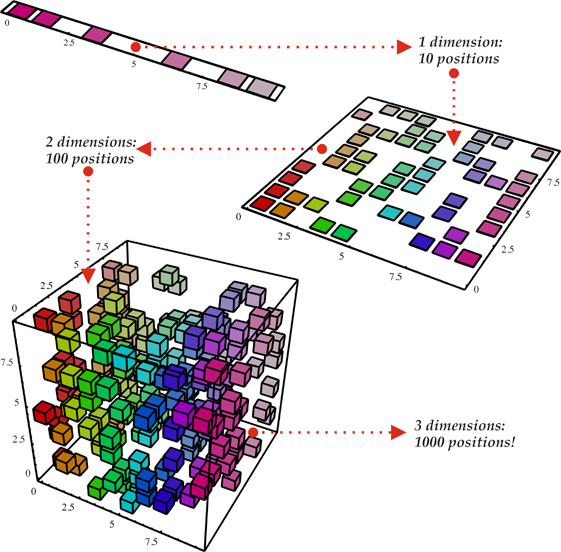
\includegraphics[width=10cm]{./textuais/desenvolvimento/figuras/CurseDimensionality.png}\\
	\caption{Demonstração gráfica da "Maldição da dimensionalidade", retirado de \cite{cursedimen}}
	\label{fig:4T01}
\end{figure}

